From the given information, for 
\begin{align}
\Vec{A} &=  \myvec{2 \\ 5 } , \Vec{B} =  \myvec{-3 \\ 6},
\vec{m} &= \vec{A}-\vec{B}
\\
& = \myvec{5 \\ -1}
\\
\implies \vec{n}& = \myvec{5 \\ -1}
\end{align}
Let 
\begin{align}
    \vec{P} = \myvec{-3\\5}
\end{align}
The equation of the desired line is then obtained as
\begin{align}
\label{linform/15/eq:line_norm_vec}
\vec{n}^T\brak{\vec{x}-\vec{P}} &= 0
\\
\implies \myvec{5 & -1} \vec{x} &= -20
\end{align}
and plotted in Fig. \ref{linform/15/fig: Perpendicular Bisector}	
\begin{figure}[!ht]
\centering
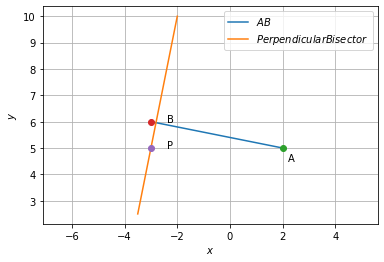
\includegraphics[width=\columnwidth]{solutions/su2021/2/15/download (6).png}
\caption{Perpendicular Bisector}
\label{linform/15/fig: Perpendicular Bisector}	
\end{figure}
